\documentclass[12pt]{book}

%These tell TeX which packages to use.
\usepackage{array,epsfig}
\usepackage{amsmath}
\usepackage{amsfonts}
\usepackage{amssymb}
\usepackage{amsxtra}
\usepackage{amsthm}
\usepackage{mathrsfs}
\usepackage{color}
\usepackage{eurosym}
\usepackage{times}
%Here I define some theorem styles and shortcut commands for symbols I use often
\theoremstyle{definition}
\newtheorem{defn}{Definition}
\newtheorem{thm}{Theorem}
\newtheorem{cor}{Corollary}
\newtheorem*{rmk}{Remark}
\newtheorem{lem}{Lemma}
\newtheorem*{joke}{Joke}
\newtheorem{ex}{Example}
\newtheorem*{soln}{Solution}
\newtheorem{prop}{Proposition}

\newcommand{\lra}{\longrightarrow}
\newcommand{\ra}{\rightarrow}
\newcommand{\surj}{\twoheadrightarrow}
\newcommand{\graph}{\mathrm{graph}}
\newcommand{\bb}[1]{\mathbb{#1}}
\newcommand{\Z}{\bb{Z}}
\newcommand{\Q}{\bb{Q}}
\newcommand{\R}{\bb{R}}
\newcommand{\C}{\bb{C}}
\newcommand{\N}{\bb{N}}
\newcommand{\M}{\mathbf{M}}
\newcommand{\m}{\mathbf{m}}
\newcommand{\MM}{\mathscr{M}}
\newcommand{\HH}{\mathscr{H}}
\newcommand{\Om}{\Omega}
\newcommand{\Ho}{\in\HH(\Om)}
\newcommand{\bd}{\partial}
\newcommand{\del}{\partial}
\newcommand{\bardel}{\overline\partial}
\newcommand{\textdf}[1]{\textbf{\textsf{#1}}\index{#1}}
\newcommand{\img}{\mathrm{omega}}
\newcommand{\ip}[2]{\left\langle{#1},{#2}\right\rangle}
\newcommand{\inter}[1]{\mathrm{int}{#1}}
\newcommand{\exter}[1]{\mathrm{ext}{#1}}
\newcommand{\cl}[1]{\mathrm{cl}{#1}}
\newcommand{\ds}{\displaystyle}
\newcommand{\vol}{\mathrm{vol}}
\newcommand{\cnt}{\mathrm{ct}}
\newcommand{\osc}{\mathrm{osc}}
\newcommand{\LL}{\mathbf{L}}
\newcommand{\UU}{\mathbf{U}}
\newcommand{\support}{\mathrm{support}}
\newcommand{\AND}{\;\wedge\;}
\newcommand{\OR}{\;\vee\;}
\newcommand{\Oset}{\varnothing}
\newcommand{\st}{\ni}
\newcommand{\wh}{\widehat}

%Pagination stuff.
\setlength{\topmargin}{-.3 in}
\setlength{\oddsidemargin}{0in}
\setlength{\evensidemargin}{0in}
\setlength{\textheight}{9.in}
\setlength{\textwidth}{6.5in}
\pagestyle{empty}

\begin{document}

\begin{center}
{\Large DATA 221 \\  Homework 4  (rev 0)}\\
\textbf{Trimble/Nussbaum}\\ %You should put your name here
Due: Friday 2023-02-03 
\end{center}

\vspace{0.2 cm}
In the last homework, you generated two lumpy distributionis that were mixtures of multivariate normal samples in 2d.
Using this distribution, we can reproduce the graph of accuracy vs model complexity of kNN classification :

% 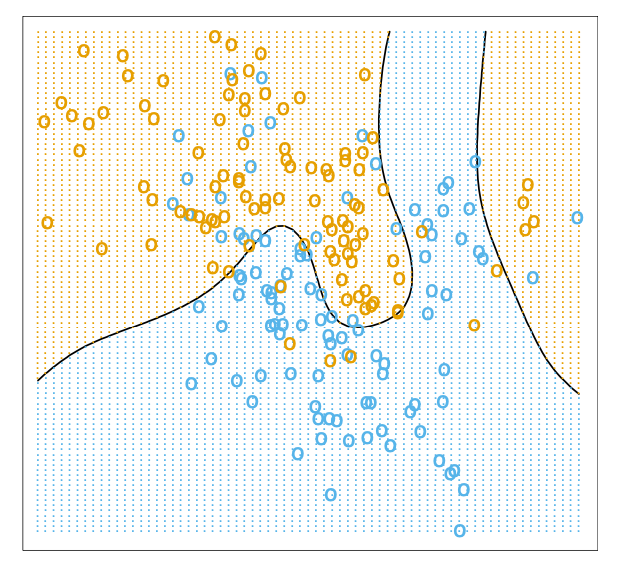
\includegraphics[width=3in]{src/hastie-bayesian.png}
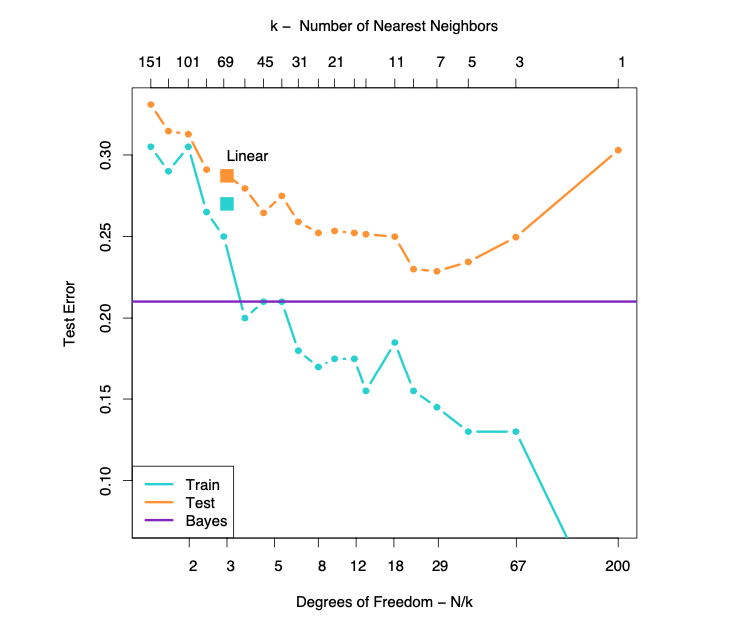
\includegraphics[width=4in]{src/hastie-generalization.png}

\begin{enumerate}
\item
Perform k-nearest-neighbor classification for at least six values of $k$ ranging from 1 to 100; use the neighbors of each point to predict the class identity.  Evaluate accuracy as a function of $k$ for the training set (with 200 points).

\item
Generate a large "testing" sample of 10,000 points from each class.  (This large set of points for evaluation causes the ${1 \over \sqrt{N} }$ sampling-based uncertainty in the correctly-classified proportion to be small, $ \sim 1\%$.) Evaluate the accuracy of KNN classification (trained on the 200-point training set)  as a function of $k$ for the 20,000 points in the test set and plot the accuracy vs. $k$ for the training and the testing data on the same graph.   


%  Looking at the UCI "default of credit card clients Data Set" contains various fields describing 30,000 credit card customers in Taiwan in 2005. (Yeh \& Lien,  doi://10.1016/j.eswa.2007.12.020)   

% \item 
%  Try to predict the \texttt{default.payment.next.month} using KNN classifiers for four different values of $k$.
% PLACEHOLDER for tuning threshold / communicating accuracy for two-category problem.

%You have to choose how to measure distance in a vector space that includes indicator variables and payment amounts (\$NT 100k).  

%Report accuracy on the testing and training datasets.

% \texttt{https://archive.ics.uci.edu/ml/datasets/default+of+credit+card+clients}

% \item
% Compare the KNN accuracy to the accuracy of logistic x 

\end{enumerate}
\end{document}


